\chapter{Image processing} \label{sec:image_processing}
\section{Image Embeddings} \label{sec:image_embeddings}
The embedding process involves transforming (encoding) a data source into a high-dimensional vector. This vector is called a \textit{vector embedding}, sometimes shortened to embedding, which refers to the final product of the embedding process. More abstractly, it is described as a mathematical function from one data space to another (representation) space $f: X \to Z$, where $X$ is the space of data, $Z$ is the space of representation, and $f$ is a function performing such a translation, see Figure \ref{fig:embedding}. In the concrete model, which describes the use case for this thesis, $X$ denotes the space of images (small binary files), $Z$ is a high-dimensional vector, and $f$ denotes the transformation model. The model is an AI model, a program trained to perform such a transformation as needed. In the process of embedding, the data source (pixels) is converted to a mathematical construct (vector); in an ideal world, the vector should contain the same information as the image itself. The most common representation of such an embedding is a high-dimensional vector whose entries are decimal (floating-point) numbers. \cite{torralba_foundations_2024}
\begin{figure}[!ht]
    \centering
    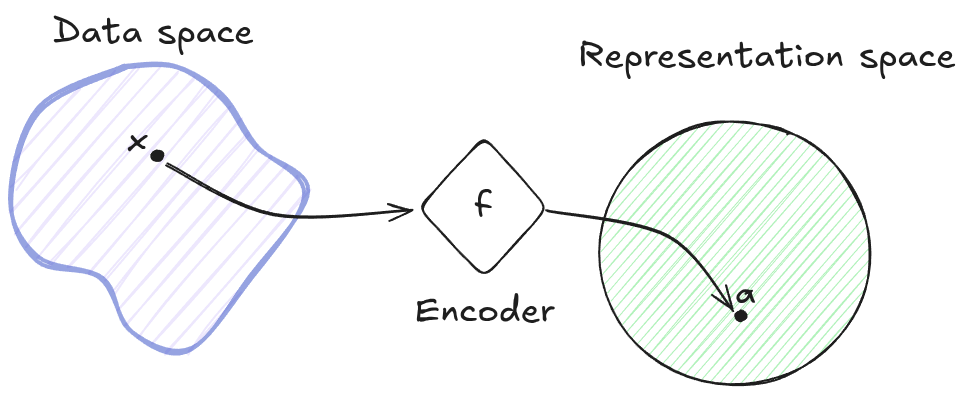
\includegraphics[width=0.75\textwidth]{images/Embeding.png}
    \caption[Embedding computations -- encode]{Embedding computations -- encode \cite{torralba_foundations_2024}}
    \label{fig:embedding}
\end{figure}

Representing data as an embedding vector creates a nice abstraction for computation. This abstraction enables computers to work with various formats in a unified manner, apply mathematical operations for processing, and, in some cases, facilitate a clearer understanding of those operations. A useful example is the indexing of such data in database systems. Having such a representation enables indexing of embeddings regardless of the data source's format.

The three main motivations for embeddings are the following:
\begin{itemize}
    \item \textbf{Compression} \\
    Embedding data can compress the original data (lossy or lossless). Such compression can reduce the storage requirements and the workload on systems that process embeddings, rather than on the original data sources.
    \item \textbf{Clearing out nuisance factors} \\
    Correctly processed information can remove data from the original source and factor out elements such as camera noise, lighting conditions, viewing angle, rotation, and others.
    \item \textbf{Decoupling} \\
    By combining the previous two features of representing raw data as embedding, it's possible to detect raw data that are either the same or hold the same information as others (according to the used model). Data projected to the same embedding can be grouped, enabling the deletion of duplicates and reducing storage and computational requirements.
    
    \cite{torralba_foundations_2024}
\end{itemize}

At the same time, embeddings entail important trade-offs. Since the mapping should also provide compression and is difficult to achieve without losing information, it must determine which factors of variation to preserve and which to discard for a given task. Different families of embeddings emphasize different visual cues and invariances, which is why various types of embeddings are suitable for a wide range of problems.

\section{Applications of Image Embeddings} \label{sec:applications_of_image_embeddings}
In the previous section, embedding is described as a process of representing data, but it is not clear which operations are suitable for such representations. One of the most well-known applications of embeddings is nearest-neighbor search. This use case employs embeddings (also known as autoencoders) to convert input data into a vector representation. Since vectors are mathematical objects on which relations such as distance can be defined and computed, those embeddings can be used to evaluate the distance between different data sources. Thanks to embedding, it is possible to define and compute distances between two sounds, images, videos, and other multimedia elements. This leads to various problems that can be addressed by understanding the distance between data sources, such as recommendation or search. The visualization of such an operation is illustrated in Figure \ref{fig:embedding_distance}.\cite{torralba_foundations_2024}
\begin{figure}[!ht]
    \centering
    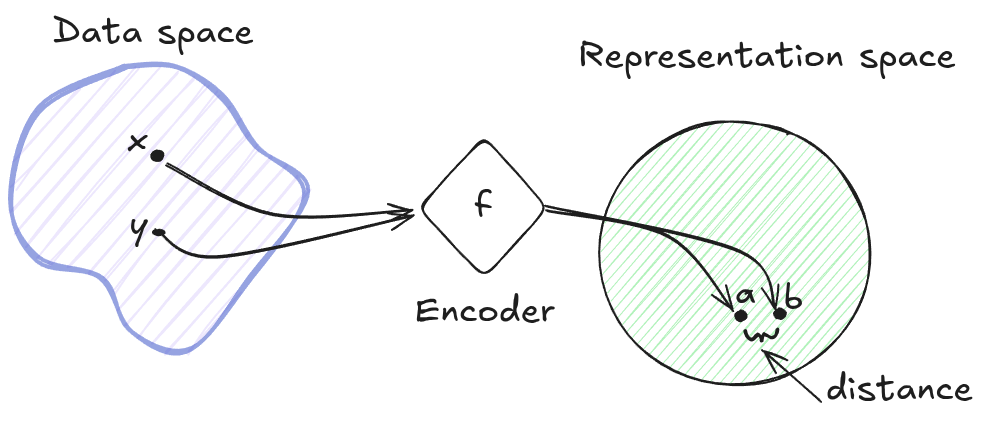
\includegraphics[width=0.75\textwidth]{images/Embeding_distance.png}
    \caption[Embedding computations -- distance]{Embedding computations -- distance \cite{torralba_foundations_2024}}
    \label{fig:embedding_distance}
\end{figure}

Another application of embeddings is predictive encoding. This is valuable for tasks such as object detection in image processing and for predicting missing data. Its use case is often seen in photo-manipulation programs, where it allows users to remove unwanted objects from the scene and replace them with elements that better fit the scene. \cite{torralba_foundations_2024}


\section{Models of Embedding Computations} \label{sec:offline_vs_online_processing}
Image-embedding systems are typically classified into two modes: online, in which embeddings are computed on demand per request, and offline, in which embeddings are precomputed and stored for later use. Both modes can coexist in real deployments, but they typically optimize very different constraints and failure risks. An example of coexistence, which also highlights the differences, is shown in Figure \ref{fig:online_offline_ec}. \cite{kiely_high-performance_2025}

\subsection{Online Processing} \label{sec:online_processing}
Online processing (also known as real-time processing) computes an image's embedding on request and returns the result with minimal additional latency. Latency is essential when the input is unknown in advance (e.g., when a user uploads an image for processing). The system must minimize queueing and cold-start effects, and enforce predictable latency, even under high traffic. To meet such requirements and optimize latency, any external dependency (e.g., remote fetches, model-weight loading) can degrade the user experience. Online pipelines, therefore, emphasize caching, admission control, and fast failure handling, accepting higher infrastructure cost to protect response times. \cite{kiely_high-performance_2025, liu_evaluation_2018}

\subsection{Offline Processing} \label{sec:offline_processing}
Offline processing (also known as batch processing) precomputes image embeddings and persists both input and output for later reuse. Images are ingested from references (typically URLs), validated as decodable media, normalized to a bounded resolution, and stored internally to eliminate reliance on unstable sources. Such computation saturates hardware efficiently and throttles as capacity dictates. The resulting vectors are linked to their source objects and model versions, enabling reproducible re-embedding when models evolve. Because offline jobs are not user-facing, the pipeline optimizes for throughput and durability rather than strict per-request latency. \cite{kiely_high-performance_2025, liu_evaluation_2018}
\begin{figure}[!ht]
    \centering
    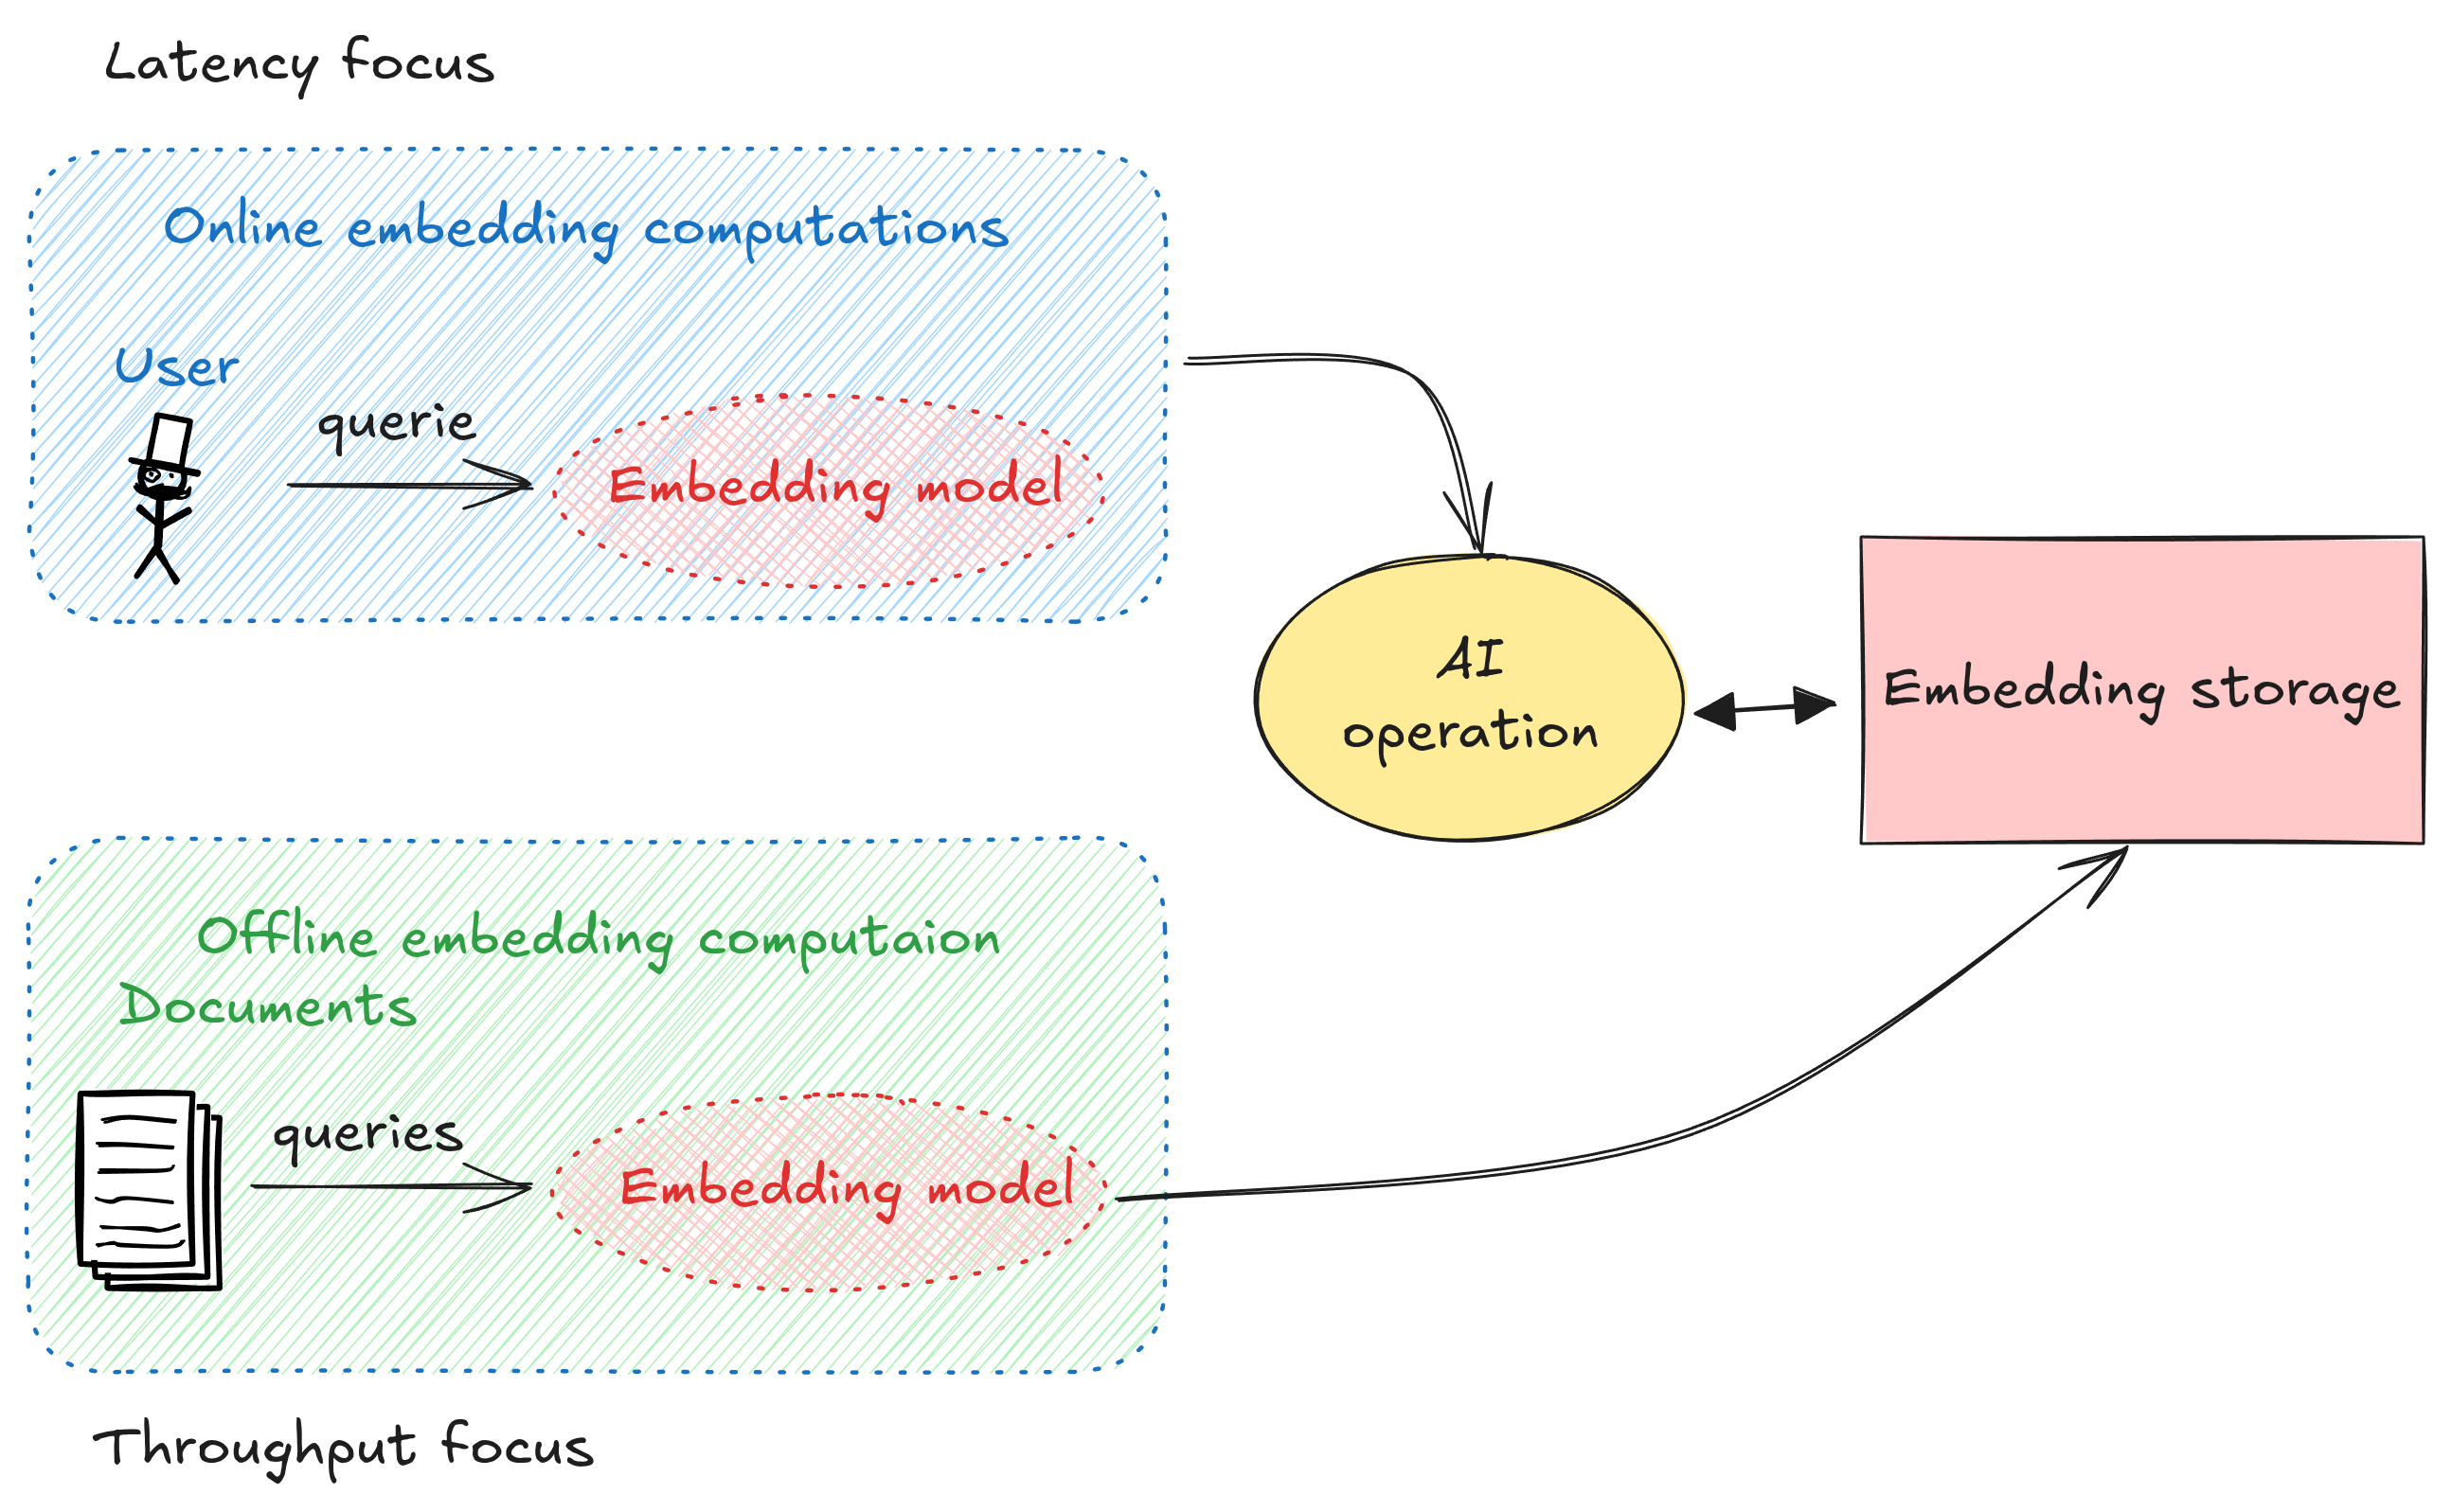
\includegraphics[width=0.75\textwidth]{images/Online_offline_ec.png}
    \caption[Online and offline embedding computation]{Online and offline embedding computation \cite{torralba_foundations_2024}}
    \label{fig:online_offline_ec}
\end{figure}

\vspace{1.5em}
Online and offline models of image processing are fundamental, often distinguished in theoretical discussions of image processing. Another model is stream processing, a hybrid of online and offline processing. It is a method that combines both throughput (from offline) and latency (from online). Such a system is the topic of this thesis. The problem of stream processing will be discussed in detail later in Chapter \ref{ch:data_processing}. For now, it is enough for the reader to be aware of the differences between online and offline processing.

\section{The Small File Problem} \label{sec:small_files_problem}
Systems that store images in the size range from $\approx 10$\,KiB to $1$\,MiB, at which this thesis is aimed, create a challenge known as the Small File Problem. This issue arises because traditional storage solutions, particularly file systems, were not designed to efficiently handle a large number of small, discrete files. The core of the problem lies in metadata overhead and file placement methods, which result in inefficiency in I/O.

Traditional file systems, such as POSIX, were designed for general-purpose single-machine use. They are tightly coupled to the operating system and store a significant amount of metadata for every file -- including permissions, ownership, timestamps (access, modification, change), and block pointers. For large files, these metadata are negligible; for small files such as images, the metadata (e.g., the inode and directory entries) can consume a disproportionately large amount of space and, more importantly, require a separate I/O operation to access.\cite{beaver_finding_2010}

This design leads to severe performance degradation at scale. To read one small file, the system must often perform multiple physical I/O operations: one or more to traverse the directory structure, another to read the file's inode (metadata), and a final one to read the actual data block. When processing millions of files, the storage subsystem is bottlenecked by these metadata-heavy random-access lookups rather than by sequential data reads. This high I/O overhead is unnecessary for ML applications, which often only need to identify a file by a unique key and retrieve its binary content. \cite{beaver_finding_2010}
